\documentclass[preview]{standalone}
\usepackage{tikz}

\begin{document}

\begin{figure}[ht]
\center
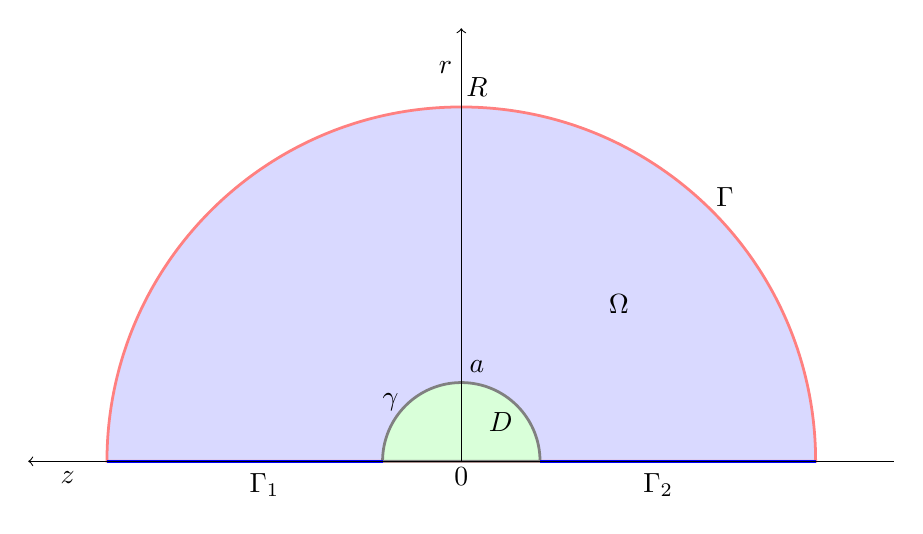
\begin{tikzpicture}[scale=1]

%    \fill [blue!15] (0,0) circle (4.5);
%    \draw [blue!50, line width=1pt] (0,0) circle (4.5);

   \fill[blue!15] (0,0) -- (0:4.5) arc (0:180:4.5) -- cycle;
   \draw [red!50, line width=1pt] (0,0) -- (0:4.5) arc (0:180:4.5) -- cycle;

   \fill[green!15] (0,0) -- (0:1) arc (0:180:1) -- cycle;
   \draw[color=black!50,line width=1pt] (0,0) -- (0:1) arc (0:180:1) -- cycle;

   \draw[color=blue,line width=1pt] (-4.5,0) -- (-1,0) (1,0) -- (4.5,0);


   \draw[<-] (-5.5,0) -- (5.5,0);
   \draw[->] (0,0) -- (0,5.5);
   \draw(0,-0.2) node {$0$};   
   \draw(-5,-0.2) node {$z$};   
   \draw(-0.2,5) node {$r$};  
   \draw(3.35,3.35) node {$\Gamma$};
   \draw(-2.5,-0.3) node {$\Gamma_1$};
   \draw(2.5,-0.3) node {$\Gamma_2$};
   \draw(0.5,0.5) node {$D$};  
   \draw(0.2,1.2) node {$a$};  
   \draw(-0.9,0.75) node {$\gamma$};
   \draw(2,2) node {$\Omega$};
   \draw(0.2,4.75) node {$R$};

 \end{tikzpicture}
\end{figure}


\end{document}